\section{Testautomatisierung}

Nach Sharma et al. ist die Testautomatisierung eine Technik,
bei der Skripte geschrieben werden, um einen manuellen
Testprozess zu automatisieren (vgl. \cite{sharma2014web}, S.909). Dabei
werden vordefinierte Tests durchgeführt, um verschiedene Funktionen in einer Anwendung zu überprüfen.
Dies bedeutet, dass Tools und Testskripte verwendet werden, um verschiedene
Zustände zu erzeugen und Daten vorzubereiten. Anschließend wird eine
Reihe von Schritten ausgeführt, um ein Szenario zu validieren.
Auf diese Weise können die Tester feststellen, ob eine Anwendung
wie erwartet funktioniert oder nicht. Entwicklungs- und Testteams
entscheiden sich aus mehreren Gründen für die Testautomatisierung.
Zu den wichtigsten gehören:

\textbf{Zeit}: Manuelle Tests sind langsam und können mit vielen Entwicklungsprozessen
nicht mithalten (vgl. \cite{sharma2014web}, S.910).


\textbf{Kosten}: Manuelle Tests sind ressourcenintensiv und kostspielig
(vgl. \cite{sharma2014web}, S.910).


\textbf{Genauigkeit}: Manuelle Tests sind bei der Durchführung sich wiederholender
Aufgaben fehleranfällig. Umgekehrt verringert die Automatisierung die
Wahrscheinlichkeit dieser Fehler (vgl. \cite{sharma2014web}, S.910).


\textbf{Umfang}: Bei der Durchführung komplexer Iterationen ist es schwierig,
sich auf manuelle Tests zu verlassen (vgl. \cite{sharma2014web}, S.910).


Laut dem Global Quality Report profitieren Unternehmen auf unterschiedliche
Weise von automatisierten Tests. Rund 60\% der Unternehmen gaben an,
dass sich die Fähigkeit zur Erkennung von Anwendungsfehlern durch eine höhere
Testabdeckung verbessert hat (vgl. \cite{Buenen201718}, S.30). Weitere 57\% stellten fest, dass die Wiederverwendung von Testfällen nach
dem Einsatz der Automatisierung zunahm. Gleichzeitig verzeichneten 54\%
eine Verringerung des Zeitaufwands für
Testzyklen (vgl. \cite{Buenen201718}, S.31).

\begin{figure}
    \centering
    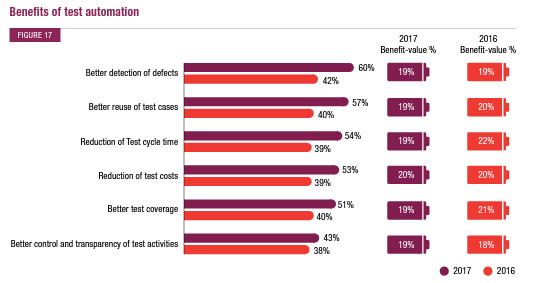
\includegraphics[scale=1.3]{images/benefits_of_test_automation}
    \caption{Vorteile der Testautomatisierung (vgl. \cite{Buenen201718}, S.31)} \label{fig:mof}
\end{figure}

In den folgenden Abschnitten werden die verschiedenen Arten von Tests
behandelt. Diese Tests können sowohl manuell als auch automatisch
durchgeführt werden. Da der Schwerpunkt dieser Arbeit auf der
Automatisierung liegt, wird nur dieser Aspekt betrachtet.
